%%%%%%%%%%%%%%%%%%%%%%%%%%%%%%%%%%%%%%%%%%%%%%%%%%%%%%%%%%%%%%%%%%%%%%%%%%%%%%%%
\subsection{Uživatelská příručka}
\subsubsection{Základní pojmy}

Nyní stručně zadefinuji základní pojmy, nutné pro pochopení fungování knihovny
ExiL a práci s ní. Význam pojmů bude jasnější, jakmile si je ukážeme na
příkladech. K těmto pojmům se posléze vrátím i~v~teoretické části textu
a~jejich popis rozšířím o další souvislosti.

První dva pojmy staví na pojmu znalost, který chápeme intuitivně a nebudu se jej
ani snažit definovat, nikoli na následujícím pojmu znalosti, jak ji chápeme
v~ExiLu (v takovém případě by byla definice cyklická).

Pojem expertního systému zatím chápejme tak, jak jsem jej představil v úvodu
práce. V teoretické části rozeberu pojem v potřebné šíři.
\begin{description}[leftmargin=6cm,style=sameline,align=right,labelsep=0.5cm]
  % \item[problémová doména] množina pojmů relevantních pro řešení určité skupiny
  %   problémů
  \item[fakt] elementární statická znalost - tvrzení
  \item[(odvozovací) pravidlo] elementární odvozovací znalost - pokud víme, že
    (ne)platí nějaká tvrzení, můžeme odvodit, že platí i~nějaká další
  \item[znalost (v ExiLu)] množina faktů a pravidel
  \item[znalostní báze] výchozí znalost expertního systému
  \item[pracovní paměť] aktuální množina faktů
  % \item[production memory] aktuální množina pravidel
  \item[inference] odvozování - postupná aplikace odvozovacích pravidel
\end{description}
Pojem \emph{pracovní paměť} není příliš intuitivní. Jde o doslovný překlad
v~literatuře užívaného pojmu \emph{working memory}, kterým je označována množina
faktů (tvrzení), které expertní systém v danou chvíli považuje za platné. Nejde
tedy ve skutečnosti o paměť, nýbrž o obsah pomyslné paměti. Pojem pracovní
množina faktů by byl jistě výstižnější, bohužel ale také značně těžkopádný.

%%%%%%%%%%%%%%%%%%%%%%%%%%%%%%%%%%%%%%%%%%%%%%%%%%%%%%%%%%%%%%%%%%%%%%%%%%%%%%%%
\subsubsection{Struktura programu}

\begin{listing}[h]
\caption{Základní struktura exilového programu}
\label{typical structure}
\begin{clcode}
;;; definition of knowledge base
;; facts
(deffacts world
  (in box A)
  (in robot B)
  (goal move box A B))

;; inference rules
(defrule move-robot
  "move robot to object's location"
  (goal move ?object ?from ?to)
  (in ?object ?from)
  (- in robot ?from)
  (in robot ?z)
  =>
  (retract (in robot ?z))
  (assert (in robot ?from)))

(defrule move-object
  "move robot and object to desired location"
  (goal move ?object ?from ?to)
  ?rob-pos <- (in robot ?from)
  ?obj-pos <- (in ?object ?from)
  =>
  (retract ?rob-pos)
  (retract ?obj-pos)
  (assert (in robot ?to))
  (assert (in ?object ?to)))

(defrule stop
  "stop if object is in desired location"
  (goal move ?object ?from ?to)
  (in ?object ?to)
  =>
  (halt))

;;; initialization of working memory
(reset)

;;; inference execution
(run)
\end{clcode}
\end{listing}

Příklad \ref{typical structure} na straně \pageref{typical structure} ukazuje
minimální strukturu programu nad knihovnou ExiL (dále exilový program). První
část programu tvoří definice znalostní báze. Ta sestává z definic faktů, ze
kterých expertní systém vychází, a definic odvozovacích pravidel, jež jsou
následně aplikována při inferenci.

Definice faktů jsou uspořádány do skupin označených názvem (v tomto případě
\verb|world|). V ukázkovém programu si snadno vystačíme s jednou skupinou faktů,
v reálných programech bude ale těchto skupin většinou více. Tato organizace
umožňuje snadnou redefinici, případně odebrání, jen některých skupin faktů v
případě potřeby. Definice skupiny faktů \verb|world| v příkladu přidává do
znalostní báze informaci o~počáteční pozici robota, krabice a~o~našem záměru
přesunout krabici z~pozice \verb|A| na pozici \verb|B|.

Následuje definice odvozovacích pravidel. Definice každého pravidla sestává z
jeho názvu, volitelného řetězce sloužícího k dokumentaci pravidla,
množiny podmínek, tedy předpokladů pro jeho splnění (a následnou aktivaci),
a~množiny důsledků, tedy libovolných lispových výrazů, které jsou při
aktivaci pravidla vyhodnoceny. Tyto dvě množiny jsou od sebe odděleny
symbolem~\verb|=>|.

Podmínky odvozovacích pravidel jsou ve formě vzorů. Struktura vzorů je stejná
jako struktura faktů (viz kapitola \ref{knowledge base definition}), ale na
rozdíl od nich mohou obsahovat proměnné (symboly začínající otazníkem). Při
vyhodnocování podmínek pravidla je zajišťěna konzistence vazeb těchto proměnných
a výskyty všech proměnných v~důsledcích pravidla jsou při jeho aktivaci
nahrazeny jejich vazbami. Detaily viz kapitola \ref{inference}

Důsledky pravidel typicky obsahují příkazy pro modifikaci pracovní paměti (viz
kapitola \ref{modifikace}), tedy přidání (\verb|assert|), odebrání
(\verb|retract|), či úpravu (\verb|modify|) faktů v ní. Nemusí tomu tak ale být
vždycky - důsledkem aktivace pravidla může být např. vypsání výstupu, logování,
zápis souboru, ale také např. ovládání externího systému.

Ukázkový příklad definuje tři odvozovací pravidla. Pravidlo
\verb|move-robot| je aktivováno, pokud chceme přesunout nějaký objekt z pozice
\verb|?from| na pozici \verb|?to|, objekt se nachází v pozici \verb|?from|
a~robot nikoli (třetí podmínka je negovaná, viz kapitola \ref{inference}).
Poslední podmínka slouží pouze k navázání původní pozice robota.  Při aktivaci
pravidla je v pracovní paměti nahrazena informace o~původní pozici robota
pozicí \verb|?from|. Robot se tedy nyní nachází na stejné pozici, jako kýžený
objekt.

Podmínky pravidla \verb|move-object| vyžadují, aby byl jak robot, tak objekt
určený k přesunu, na pozici \verb|?from|. Při jeho aktivaci je robot i s objektem
přesunut na pozici \verb|?to| nahrazením faktů o původních pozicích novými,
podobně jako v~prvním pravidle. Definice pravidla obsahuje speciální notaci (s
použitím operátoru \verb|<-|), jejímž účelem je navázání celého faktu na
proměnnou. Ten pak můžeme v~důsledcích snadno ostranit z pracovní paměti.
Detaily opět viz kapitola \ref{inference}

Poslední pravidlo slouží k zastavení inference, pokud se již objekt nachází na
cílové pozici. Inference je zde zastavena explicitním voláním \verb|(halt)|.
Druhou možností by bylo odstranit z pracovní paměti fakt definující cíl (jak
vidíme v~příkladu \ref{structured facts}), neboť v takovou chvíli nemůže být
žádné další pravidlo splňeno.

Jakmile je znalostní báze nadefinována, můžeme z ní inicializovat pracovní
paměť. To provedeme voláním \verb|(reset)|, které, po případném vymazání
původních faktů, přidá do pracovní paměti fakty ve všech definovaných skupinách.

Poslední nutnou fází exilového programu je spuštění inference. To můžeme udělat
nejjednodušeji voláním \verb|(run)|. Inferenční mechanismus poté postupně
vyhodnocuje, která odvozovací pravidla mají splněné všechny podmínky, v každém
kroku z nich jedno vybere a aktivuje jej. Detaily viz kapitola \ref{inference}

Výstup programu je následující:
\begin{minted}{cl}
==> (IN ROBOT B)
==> (IN BOX A)
==> (GOAL MOVE BOX A B)
Firing MOVE-ROBOT
<== (IN ROBOT B)
==> (IN ROBOT A)
Firing MOVE-OBJECT
<== (IN ROBOT A)
<== (IN BOX A)
==> (IN ROBOT B)
==> (IN BOX B)
Firing STOP
Halting
\end{minted}
Řádky začínající symbolem \verb|==>| označují fakty přidané do pracovní paměti,
řádky začínající \verb|<==| fakty z paměti odstraněné. Tento výstup obdržíme
pouze pokud zapneme sledování faktů voláním \verb|(watch facts)| (viz kapitola
\ref{inference tracing}). První tři fakty přibydou do pracovní paměti při
vyhodnocení volání \verb|(reset)|, další pak s~postupnou aplikací
odvozovacích pravidel. Dotážeme-li se po skončení inference na seznam faktů v
pracovní paměti voláním \verb|(facts)|, obdržíme výstup
\cl|((GOAL MOVE BOX A B) (IN ROBOT B) (IN BOX B)).|
Robot i krabice jsou tedy na cílové pozici.

Kód exilového programu má deklarativní charakter. Nikde jsme nemuseli
specifikovat, jakou posloupností akcí má systém k výsledku dospět. To nás ovšem
nezbavuje nutnosti chápat fungování inferenčního mechanismu ExiLu. Nebudeme-li
při konstrukci programu opatrní, může výpočet snadno dospět k neočekávaným
výsledkům, dostat se do slepé větve, či se zacyklit. Tyto problémy jsou často
způsobeny nezamýšlenou interferencí podmínek pravidel s důsledky jiných.

\FloatBarrier

Skupina pravidel může například snadno cyklit, pokud první pravidlo závisí na
neexistenci nějakého faktu, tento v důsledcích přidá, načež je tento fakt
posledním pravidlem odstraněn, aniž by byla v průběhu zneplatněna nějaká další
podmínka prvního pravidla. Fakt, který odvodíme v jedné část programu může také
neočekávaně splnit podmínku pravidla definovaného v úplně jiné části, která s
první neměla vůbec přímo komunikovat.

\subsubsection{Definice znalostní báze}
\label{knowledge base definition}

ExiL, stejně jako CLIPS, rozlišuje dva typy faktů - jednoduché (\emph{simple,
ordered}) a strukturované (\emph{templated}). Stuktura jednoduchého faktu je udána
pouze pořadím atomů, typickou volbou je např. \verb|objekt-attribut-hodnota|:
\cl|(box color red),| či \verb|relace-objekty|: \cl|(in box hall).|

Strukturované fakty mají naproti tomu explicitně pojmenované složky (sloty).
Typicky popisují objekt s pojmenovanými atributy:
\cl|(box :color red :size small),| či relaci s pojmenovanými zůčastněnými
objekty: \cl|(in :object box :location hall),| kde \verb|box| a \verb|in| jsou
šablony (\emph{template}), které je třeba definovat předem. Na pořadí
specifikace slotů u strukturovaných faktů nezáleží.

Vyjadřovací síla obou typů faktů je stejná, použitím explicitnějších
strukturovaných faktů ale docílíme lepší čitelnosti a jednoznačnější sémantiky
exilového programu, zvláště třeba v případě relací na jedné množině objektů:
\cl|(father john george).|

Šablonu definujeme voláním makra \verb|deftemplate|, např:
\cl|(deftemplate in object (location :default here)).| Prvním parametrem je
název šablony, za ním následuje libovolný počet specifikací slotů. Specifikací
slotu je buď symbol - jméno slotu, nebo \emph{seznam}, jehož hlavou
(\emph{car}) je jméno slotu a~tělem (\emph{cdr}) je \emph{property list (plist)}
s dalšími parametry. Aktuálně systém umožňuje pouze specifikaci výchozí hodnoty
slotu \emph{klíčkem} \verb|:default|. Ta je použita, není-li při specifikaci
faktu, používajícího tuto šablonu, uvedena hodnota pro daný slot. Příklad
\ref{structured facts} na straně \pageref{structured facts} ukazuje definici
znalostní báze ekvivalentní příkladu \ref{typical structure} s použitím
strukturovaných faktů.

\begin{listing}[h]
\caption{Definice znalostní báze s použitím strukturovaných faktů}
\label{structured facts}
\begin{clcode}
(deftemplate goal (action :default move) object from to)
(deftemplate in object location)

(deffacts world
  (in :object robot :location A)
  (in :object box :location B)
  (goal :object box :from B :to A))

(defrule move-robot
  (goal :object ?obj :from ?from)
  (in :object ?obj :location ?from)
  (- in :object robot :location ?from)
  ?robot <- (in :object robot :location ?)
  =>
  (modify ?robot :location ?from))

(defrule move-object
  (goal :object ?obj :from ?from :to ?to)
  ?object <- (in :object ?obj :location ?from)
  ?robot <- (in :object robot :location ?from)
  =>
  (modify ?robot :location ?to)
  (modify ?object :location ?to))

(defrule stop
  ?goal <- (goal :object ?obj :to ?to)
  (in :object ?obj :location ?to)
  =>
  (retract ?goal))
\end{clcode}
\end{listing}

Je-li už šablona požadovaného názvu definována, ale neexistují v pracovní
paměti fakty, které ji používají, je její stávající definice nahrazena. Pokud
ale v~pracovní paměti nebo v některé z definic skupin faktů existují takové
fakty, skončí volání \verb|deftemplate| výjimkou.

Seznam názvů všech definovaných šablon můžeme získat voláním \verb|(templates)|.
Specifikaci šablony pak získáme voláním makra
\verb|find-template|, např. \verb|(find-template in).| Definici šablony zrušíme
voláním makra \verb|undeftemplate|, např. \verb|(undeftemplate goal)|. To opět
skončí výjimkou, existují-li v pracovní paměti nebo v některé ze skupin fakty,
které šablonu využívají.

Fakty, ze kterých expertní systém vychází, zavádíme pomocí skupin faktů. Ty
definujeme makrem \verb|deffacts|, např.:
\begin{minted}{cl}
(deffacts initial
  (goal move box A B)
  (in :object box :location A))
\end{minted}
Prvním parametrem je název skupiny, pak následuje libovolný počet specifikací
faktů. Opakovaným voláním makra \verb|deffacts| je skupina faktů
redefinována.

Specifikace faktu je vždy tvořena seznamem. Pokud jde o jednoduchý fakt,
specifikací je prostě seznam atomů. Jde-li o fakt strukturovaný, je prvním
prvkem specifikace název šablony, za ním následuje plist určující hodnoty slotů
faktu. Pokud není hodnota některého slotu uvedena, je buď použita
výchozí hodnota, pokud byla v šabloně specifikována, nebo hodnota \verb|nil| v
opačném případě.

Seznam názvů všech definovaných skupin faktů získáme voláním
\verb|(fact-groups)|. Specifikaci skupiny pak voláním makra
\verb|find-fact-group|, např. \verb|(find-fact-group initial)|. Ke zrušení
definice skupiny slouží makro \verb|undeffacts| (voláme s názvem skupiny).

Pravidla, pomocí nichž expertní systém během inference odvozuje nové fakty,
definujeme makrem
\verb|defrule|, např.:
\begin{minted}{cl}
(defrule move-robot
  "move robot to object's location"
  (goal :action move :object ?obj :from ?from)
  (in :object ?obj :location ?from)
  (- in :object robot :location ?from)
  ?robot <- (in :object robot :location ?)
  =>
  (modify ?robot :location ?from)).
\end{minted}
Podmínková část pravidla (před symbolem \verb|=>|) je tvořena vzory. Ty mohou
být, stejně jako fakty, jednoduché nebo strukturované. Kromě toho umožňuje
definice pravidla několik speciálních konstruktů (negace podmínky, navázání
proměnné na celou podmínku). Ty popíšu podrobně v kapitole \ref{inference} spolu~s
tím, jak jsou podmínky pravidla při inferenci vyhodnocovány.

\FloatBarrier

Důsledkovou část pravidla (za symbolem \verb|=>|) tvoří libovolný počet
lispových výrazů. Jak se tyto vyhodnocují popíšu opět v kapitole \ref{inference}

Opakovaným voláním makra \verb|defrule| odvozovací pravidlo redefinujeme.
K~získání seznamu názvů definovaných pravidel a jejich specifikací slouží
funkce \verb|rules| a makro \verb|find-rule|, podobně jako u šablon a
skupin faktů.  Ke zrušení definice pravidla slouží makro \verb|undefrule|.

\subsubsection{Modifikace pracovní paměti}
\label{modifikace}

Pracovní paměť je množina faktů, které systém v danou chvíli považuje za platné.
Její obsah můžeme vypsat voláním funkce \verb|facts|. Funkcí \verb|reset|
inicializujeme pracovní paměť ze znalostní báze. Jejím voláním jsou do pracovní
paměti zavedeny fakty všech definovaných skupin faktů (viz kapitola
\ref{knowledge base definition}).

Obsah pracovní paměťi může být dále modifikován třemi makry:
\begin{itemize}
  \item \verb|assert| přidává fakt(y) do pracovní paměti,
  \item \verb|retract| fakt(y) z pracovní paměti odebírá a
  \item \verb|modify| přímo modifikuje existující fakt.
\end{itemize}
Ta lze volat buď před započetím inference (ale po volání \verb|reset|, neboť to
pracovní paměť vymaže), nebo v jejím průběhu, pokud inferenci krokujeme (viz
kapitola \ref{inference}). Makra také typicky voláme v důsledcích pravidel.

Makra \verb|assert| a \verb|retract| berou jako parametry libovolný počet
specifikací faktů ve stejném formátu, jako u makra \verb|deffacts| (ale bez
názvu skupiny). Makro \verb|modify| lze použít jen u strukturovaných faktů. Toto
makro bere jako první parametr specifikaci faktu, zbytek parametrů tvoří plist
určující hodnoty slotů ke změně. Například volání
\begin{minted}{cl}
(modify (in :object box :location A) :location B)
\end{minted}
nahradí v pracovní paměti fakt \verb|(in :object box :location A)| faktem
\verb|(in :object box :location B)|.
Toto makro je obzvláště užitečné, navážeme-li v podmínkách pravidla celý fakt na
proměnnou (viz kapitola \ref{inference}).

Pracovní paměť se skutečně chová jako množina, každý fakt tedy může být v
pracovní paměti jen jednou. Opětovné volání \verb|assert| nemá žádný efekt.
Volání modify, jehož výsledkem by bylo nahrazení nějakého faktu faktem, který
již v~pracovní paměti existuje, sice odebere původní fakt, nový však znovu
nepřidá.

Všechny fakty můžeme z pracovní paměti odebrat voláním \verb|(retract-all)|. To
je ale zřídka užitečné, typicky použijeme spíše funkci \verb|reset| pro
navrácení pracovní paměti do výchozího stavu, tedy reinicializaci ze znalostní
báze.

\subsubsection{Inference}
\label{inference}

Inference (odvozování nových faktů z aktuálních) probíhá v krocích. V každém
kroku jsou vyhodnoceny podmínky všech pravidel, načež je ze splněných pravidel
vybráno jedno, které je posléze aktivováno. Inferenční kroky můžeme buď spouštět
jednotlivě voláním \verb|(step)|, nebo voláním \verb|(run)| spustit
cyklus, který provádí inferenční kroky, dokud je to možné. Cyklus je buď
přerušen ve chvíli, kdy není splněno žádné další pravidlo, nebo voláním
\verb|(halt)| v důsledcích právě aktivovaného pravidla.

Podmínky pravidel jsou ve tvaru vzorů a jsou spojeny logickou konjunkcí,
pravidlo je tedy splněno, jsou-li splněny všechny jeho podmínky. Kromě
toho mohou být některé podmínky negovány. Taková podmínka je splněna tehdy,
neexistuje-li v pracovní paměti žádný fakt, který by se shodoval s jejím vzorem
(při zachování konzistence vazeb proměnných). Negovanou podmínku značí znak
\verb|-| (minus) na prvním místě specifikace vzoru.

Vyhodnocování podmínek pravidel probíhá ve dvou fázích. V první fází srovnáváme
vzory jednotlivých podmínek se všemi fakty v pracovní paměti a~to pouze
strukturálně, tedy bez ohledu na vazby proměnných. Prvním požadavkem shody je u
jednoduchých faktů stejná délka (počet atomů), u strukturovaných faktů stejná
šablona. Jednoduchý fakt se nikdy nemůže shodovat se strukturovaným vzorem a
naopak.

Dále jsou pak porovnávány jednotlivé atomy (u jednoduchých) či
sloty (u~složených) faktu vůči odpovídajícímu atomu (slotu) vzoru. Není-li atom
(slot) vzoru proměnná, je jednoduše porovnán s atomem faktu. Je-li atomem
proměnná, považujeme jej v této fázi automaticky za shodu. Například vzor
\cl|(in :object robot :location ?loc)|
se shoduje s faktem
\cl|(in :object robot :location A)|
nikoli však s fakty
\begin{minted}{cl}
(in :object box :location A)
(is-in :object robot :location A)
(in robot A).
\end{minted}
Tímto předvýběrem
tedy získáme ke každé podmínce pravidla množinu faktů, které mají stejnou
strukturu a stejné hodnoty neproměnných atomů.

Ve druhé fázi vyhodnocování hledáme z předvybraných faktů takovou posloupnost
(délka odpovídá počtu podmínek pravidla), kde po spárování s odpovídajícími
vzory podmínek obdržíme konzistentní vazby proměnných. To znamená, že
vyskytuje-li se v podmínkách pravila některá proměnná vícekrát, musí mít
odpovídající fakty na daných pozicích stejný atom.  Mějme například pravidlo
s~podmínkami
\begin{minted}{cl}
(goal move ?obj ?from ?to)
(in :object ?obj  :location ?from)
(in :object robot :location ?to)
\end{minted}
Vzor první podmínky je jednoduchý, zatímco další dva jsou strukturované. To ale
ničemu nevadí, je třeba pouze najít fakty odpovídající struktury. Posloupnost
faktů
\begin{minted}{cl}
(goal move box A B)
(in :object box   :location B)
(in :object robot :location A)
\end{minted}
neprojde druhou fází výběru, neboť vazby proměnných nejsou konzistentní.
Proměnná \verb|?from| je například v první podmínce navázána na symbol \verb|A|, v
druhé ale na \verb|B|. Kdyby si ovšem krabice s robotem vyměnily pozice, budou
vazby proměnných konzistentní a podmínky pravidla budou splněny. Proměnná
\verb|?from| by pak nabyla hodnoty \verb|A|, proměnná \verb|?to| hodnoty
\verb|B| a proměnná \verb|?obj| hodnoty \verb|box|.

Vyhodnocení negovaných podmínek si můžeme představit tak, že nejprve vyhodnotíme
a navážeme proměnné všech ostatních podmínek. Pokud poté neexistuje fakt, který
by se se vzorem negované podmínky shodoval a měl konzistentní vazby se zbytkem navázaných
proměnných, je tato podmínka splněna. Mějme například pravidlo s~podmínkami
\begin{minted}{cl}
(goal move box ?from ?to)
(in box ?from)
(- in robot ?from).
\end{minted}
Máme-li v pracovní paměti pouze fakty
\begin{minted}{cl}
(goal move box A B)
(in box A)
(in robot B),
\end{minted}
budou podmínky pravidla splněny, neboť po spárování vzorů prvních dvou podmínek
s prvními dvěma fakty bude proměnná \verb|?from| navázána na hodnotu
\verb|A|~a~neexistuje fakt, který by se shodoval se vzorem \verb|(in robot A)|.
Přesuneme-li ale robota na pozici \verb|A|, podmínka již splněna nebude a
pravidlo nelze aktivovat.

Ve vzorech podmínek pravidla můžeme využít speciální proměnné \verb|?|.
Konzistence vazby této proměnné není při vyhodnocování testována, takže
vyskytuje-li se tato proměnná na více místech, chová se tak, jako kdyby byl
každý výskyt označen unikátním názvem (podobně jako proměnná \verb|_| v
Prologu). Použitím této proměnné dáváme najevo, že nás konkrétní hodnota daného
atomu nazajímá. Ve strukturovaných vzorech podmínek není třeba tyto sloty uvádět,
neboť \verb|?| je výchozí hodnotou slotu vzoru.

Posledním speciálním konstruktem je navázání celého faktu na proměnnou.
Například pravidlo
\begin{minted}{cl}
(defrule move
  ?fact <- (in :object ? :location A)
  =>
  (modify ?fact :location B))
\end{minted}
přesune každý objekt z pozice \verb|A| na pozici \verb|B|. Na proměnnou
můžeme navázat i~jednoduchý fakt, pak ale nemůžeme použít makra \verb|modify|.
Můžeme ovšem volat \verb|(retract ?fact)|, neboť proměnná \verb|?fact| je při
aktivaci pravidla nahrazena specifikací faktu, který byl se vzorem podmínky
spárován.

Podmínky některých pravidel mohou být při vyhodnocování splněny několika různými
posloupnostmi faktů. Výsledkem vyhodnocování pravidel tedy není pouze množina
splněných pravidel, nýbrž množina shod (\emph{match}). Každá shoda je tvořena
pravidlem a \emph{subsitucí} proměnných navázaných při vyhodnocování jeho
podmínek.  Subsituci chápejme jako zobrazení z množiny všech proměnných,
vyskytujících se v podmínkách pravidla, na konkrétní hodnoty atomů (slotů).
Aplikací této substituce na vzory podmínek pravidla získáme opět posloupnost
faktů, kterými byly podmínky v dané shodě splněny. Tato substituce je následně
použita při aktivaci pravidla k náhradě proměnných v jeho důsledích.

ExiL uchovává aktuální množinu shod. Ta ve skutečnosti není přepočítána v~první
fázi inferenčního kroku, jak jsem dosud pro jednoduchost tvrdil, nýbrž
automaticky po každé změně pracovní paměti či množiny pravidel (detaily viz
RETE).  Aktuální množinu shod nazývám, po vzoru CLIPSu, \emph{agenda} a lze ji
vypsat voláním stejnojmenné funkce. Každá shoda v agendě je opatřena časovým
razítkem, shody je tedy možné uspořádat podle toho, kdy do agendy přibyly.

Je-li na začátku inferenčního kroku v agendě více shod, je třeba z nich jednu
vybrat k aktivaci. Výběr shody záleží na zvolené strategii. ExiL poskytuje
následující strategie výběru shody:
\begin{description}[leftmargin=5cm,style=sameline,align=right,labelsep=0.5cm]
  \item[depth-strategy] vybírá shodu, která do agendy přibyla nejpozději
  \item[breadth-strategy] vybírá shodu, která do agendy přibyla jako první
  \item[simplicity-strategy] vybere shodu, jejíž pravidlo má nejméně podmínek
  \item[complexity-strategy] volí shodu, jejíž pravidlo má nejvíce podmínek.
\end{description}
Názvy prvních dvou strategií vychází z toho, že jde o prohledávání prostoru
stavů systému do hloubky, či do šířky, jak blíže popíšu v teoretické části
textu, spolu s~motivacemi pro využití jednotlivých typů strategií a dalšími typy
strategií, které se v expertních systémech používají.

Výchozí strategií je \verb|depth-strategy|. Strategii, která bude v inferenci
použita, můžeme zvolit voláním makra \verb|setstrategy| s názvem strategie,
např. \verb|(setstrategy breadth-strategy)|. Seznam názvů strategií můžeme
vypsat voláním \verb|(strategies)|, název aktuálně zvolené strategie pak voláním
\verb|(current-strategy)|.

Po výběru shody k aktivaci je její pravidlo aktivováno. Nejprve jsou v
důsledcích pravidla nahrazeny všechny proměnné pomocí substituce shody. Výrazy
v~důsledcích jsou poté vyhodnoceny lispovým makrem \verb|eval|. Tento způsob
vyhodnocení vede ke značným omezením. Výrazy totiž nejsou vyhodnoceny v
\emph{lexikálním prostředí} definice pravidla, nýbrž ve výchozím (\emph{top-level})
prostředí Lispu. Díky tomu nemůžeme v důsledcích pravidla volat lokální funkce
(definované např. makrem \verb|labels|), či přistupovat k lokálním proměnným
(navázaným například v~\verb|let|u či pomoci \emph{destrukturujících maker}).

V důsledcích každého pravidla chceme typicky alespoň jednou volat některé
z~maker modifikujících pracovní paměť, abychom zneplatnili podmínky pravidla,
jinak se inference zacyklí. Druhou možností je přerušit inferenci voláním
\verb|(halt)|. Volání \verb|(step)| nebo \verb|(run)| ve chvíli, kdy již nelze
dále odvozovat (žádné z pravidel nemá splněné podmínky), nemá žádný efekt.

%%%%%%%%%%%%%%%%%%%%%%%%%%%%%%%%%%%%%%%%%%%%%%%%%%%%%%%%%%%%%%%%%%%%%%%%%%%%%%%%
\subsubsection{Sledování průběhu inference}
ExiL umožnuje sledovat několik typů událostí, ke kterým dochází během inference.
K nastavení sledovaných událostí slouží makra \verb|watch| a \verb|unwatch|. K
zjištění stavu sledování pak makro \verb|watchedp|.

Základním výstupem programu \ref{typical structure} na straně \pageref{typical
structure} je
\begin{minted}{cl}
Firing MOVE
Firing PUSH
Firing STOP
Halting.
\end{minted}
Zapneme-li sledování faktů voláním \verb|(watch facts)|, obdržíme výstup
\begin{minted}{cl}
==> (IN BOX A)
==> (IN ROBOT B)
==> (GOAL MOVE BOX A B)
Firing MOVE-ROBOT
<== (IN ROBOT B)
==> (IN ROBOT A)
Firing MOVE-OBJECT
<== (IN ROBOT A)
<== (IN BOX A)
==> (IN ROBOT B)
==> (IN BOX B)
Firing STOP
Halting.
\end{minted}

Sledování pravidel (\verb|(watch rules)|), přidává informace o pravidel
přidaných do (odebraných ze) znalostní báze, např.
\begin{minted}{cl}
==> (RULE STOP
  (GOAL MOVE ?OBJECT ?FROM ?TO)
  (IN ?OBJECT ?TO)
  =>
  (HALT)).
\end{minted}

Po zapnutí sledování agendy (voláním \verb|(watch activations)|, název je kvůli
kompatibilitě se systémem CLIPS) budeme navíc informováni o shodách, které do
agendy přibyly, nebo z ní byly odstraněny. Výstup programu pak bude následující:
\begin{minted}[samepage]{cl}
==> (MATCH MOVE-ROBOT
      ((GOAL MOVE BOX A B) (IN BOX A) (IN ROBOT B)))
Firing MOVE-ROBOT
==> (MATCH MOVE-OBJECT
      ((GOAL MOVE BOX A B) (IN BOX A) (IN ROBOT A)))
==> (MATCH MOVE-ROBOT
      ((GOAL MOVE BOX A B) (IN BOX A) (IN ROBOT A)))
<== (MATCH MOVE-ROBOT
      ((GOAL MOVE BOX A B) (IN BOX A) (IN ROBOT A)))
Firing MOVE-OBJECT
==> (MATCH STOP ((GOAL MOVE BOX A B) (IN BOX B)))
Firing STOP
Halting.
\end{minted}
Každá shoda je zde reprezentována názvem pravidla a posloupností faktů, které
byly spárovány s jeho podmínkami. Odtud můžeme snadno odvodit substituci, jež
byla při vyhodnocení použita. Negované podmínky nejsou spárovány s žádným
konkréním faktem, proto jsou zde jen tři fakty, přestože pravidlo
\verb|move-robot| má podmínky čtyři.

Je zde také vidět, že po aktivaci pravidla
\verb|move-robot| se v agendě na chvíli objeví opětovná shoda tohoto pravidla.
To je způsobeno tím, že obsah agendy se přepočítává po každé změně pracovní
paměti, takže se zde mohou objevit dočasné výsledky.

%%%%%%%%%%%%%%%%%%%%%%%%%%%%%%%%%%%%%%%%%%%%%%%%%%%%%%%%%%%%%%%%%%%%%%%%%%%%%%%%
\subsubsection{Undo/redo}

Jedním z implementovaných rozšíření původního programu je schopnost vrácení
provedených změn. K tomu slouží makra \verb|undo| a \verb|redo|. Ta lze použít k
vrácení jakékoli akce s vedlejším efektem, včetně kroků inference. K vypsání
zásobníků s~akcemi, které je možné vrátit, jsou k dispozici makra
\verb|undo-stack| a \verb|redo-stack|.

Pokud například vyhodnotíme prvních 32 řádků programu \ref{typical structure} na
straně \pageref{typical structure} a~zavoláme dvakrát \verb|undo|, bude výpis
zásobníků následující (přeformátováno):
\begin{minted}[samepage]{cl}
EXIL-USER> (undo-stack)
  1: (defrule MOVE-ROBOT
       ((GOAL MOVE ?OBJECT ?FROM ?TO)
        (IN ?OBJECT ?FROM)
        (- IN ROBOT ?FROM) (IN ROBOT ?Z)
        =>
        (RETRACT (IN ROBOT ?Z))
        (ASSERT (IN ROBOT ?FROM))))
  2: (deffacts WORLD
       ((IN BOX A) (IN ROBOT B) (GOAL MOVE BOX A B)))
\end{minted}
\begin{minted}[samepage]{cl}
EXIL-USER> (redo-stack)
  1: (defrule MOVE-OBJECT
       ((GOAL MOVE ?OBJECT ?FROM ?TO)
        ?OBJ-POS <- (IN ?OBJECT ?FROM)
        ?ROB-POS <- (IN ROBOT ?FROM)
        =>
        (RETRACT ?ROB-POS)
        (RETRACT ?OBJ-POS)
        (ASSERT (IN ROBOT ?TO))
        (ASSERT (IN ?OBJECT ?TO))))
  2: (defrule STOP
       ((GOAL MOVE ?OBJECT ?FROM ?TO)
        (IN ?OBJECT ?TO)
        =>
        (HALT)))
\end{minted}
Vidíme tedy, že jsme vrátili zpět definice pravidel \verb|move-object| a
\verb|stop| (ty bychom mohli opět provést voláním \verb|(redo)|). Dalším voláním
\verb|(undo)| by pak byla vrácena definice pravidla \verb|move-robot| a poté
definice skupiny faktů \verb|world|.

Nemá-li akce žádný vedlejší efekt - např. volání \verb|assert| s faktem, který
už v~pracovní paměti je, či volání \verb|run| ve chvíli, kdy už není co
odvozovat - prázdná akce se na zásobník neuloží.

\begin{framed}
zvážit, zda popis chování undo + reset patří sem, nebo do resetu prostředí
\end{framed}

%%%%%%%%%%%%%%%%%%%%%%%%%%%%%%%%%%%%%%%%%%%%%%%%%%%%%%%%%%%%%%%%%%%%%%%%%%%%%%%%
\subsubsection{Zpětná inference}
\label{backward inference}

Dalším z implementovaných rozšíření je možnost zpětné inference. Inference
popsaná v kapitole \ref{inference} je dopředná. V každém kroku jsou nalezeny
všechny možnosti dalšího postupu odvozování, načež je zvolena jedna, kterou se
program dále ubírá. To činí průběh inference značně nedeterministickým. Možnosti
postupu, které nebyly vybrány, mohou být navíc dalším postupem ztraceny, pokud
aktivace některého pravidla zneplatní podmínky jiného.
Míru nedeterminismu můžeme snížit tím, že budeme navrhovat odvozovací pravidla
tak, aby se výpočet neubíral nechtěnými cestami. To ale není vždy jednoduché,
nebo dokonce možné.

Zpětná inference naproti tomu umožňuje definovat cíle, kterých chceme dosáhnout.
K tomu slouží makro \verb|defgoal|, kterému předáme vzor ve stejném formátu,
jako u podmínek pravidel. Definice cíle ovšem nepodporuje negaci ani navázání
faktu na proměnnou (k tomu ani není důvod). Cíle je pak možné vypsat voláním
\verb|(goals)|. Cíl můžeme také odebrat makrem \verb|undefgoal|.
Ke spuštění zpětné inference slouží funkce \verb|back-step| a
\verb|back-run|, podobně jako u inference dopředné.

Mějme následující znalostní bázi:
\begin{minted}{cl}
(deffacts world
  (have-money))

(defrule buy-car
  (have-money)
  =>
  (retract (have-money))
  (assert (have-car)))

(defrule pay-rent
  (have-money)
  =>
  (retract (have-money))
  (assert (rent-payed))).
\end{minted}
Spustíme-li dopřednou inferenci, systém nám vesele doporučí nákup auta.
Mít nové auto je sice pěkné, hrozí-li nám ale vykázání z pronajatého bytu,
není nákup auta pravděpodobně cestou, kterou bychom se chtěli ubírat.
Systém by nám v tuto chvíli mohl stejně dobře doporučit správnou cestu. Že bylo
vybráno zrovna první pravidlo je výsledkem toho, jak funguje síť RETE, která
pravidla vyhodnocuje. Za daných okolností ale nechceme špatnou variantu ani
připouštět.

V tomto případě bychom mohli upravit definici programu tak, že do znalostní báze
přidáme informaci o cíli, kterou budou pravidla zohledňovat, podobně jako
v~příkladu \ref{typical structure} na straně \pageref{typical structure}. Muset
ale programovat zohlednění cíle v každém pravidle je přinejmenším otravné. U
větších programů to navíc může být velmi náročné, neboť cíl bude třeba
programově modifikovat v průběhu výpočtu.

S použitím zpětné inference je problém podstatně jednodušší. Zavoláme-li
\begin{minted}{cl}
(reset)
(defgoal (rent-payed))
(back-run),
\end{minted}
bude výsledkem výstup
\begin{minted}[samepage]{cl}
All goals have been satisfied
(RENT-PAYED) satisfied by (RULE PAY-RENT
  (HAVE-MONEY)
  =>
  (RETRACT (HAVE-MONEY))
  (ASSERT (RENT-PAYED)))
(HAVE-MONEY) satisfied by (HAVE-MONEY).
\end{minted}
Zde vidíme, že po spuštění zpětné inference nezačal systém bezhlavě provádět
akce, ke kterým měl dostatečné prostředky. Místo toho systém uvážil zadaný cíl a
jal se hledat akce, které k vedou jeho splnění.

Uvažme nyní složitější příklad (definice šablon vynechána):
\begin{minted}[samepage]{cl}
(deffacts world
  (female jane)
  (male john)
  (parent :parent jane :child george)
  (parent :parent john :child george))

(defrule father-is-male-parent
  (male ?father)
  (parent :parent ?father :child ?child)
  =>
  (assert (father :father ?father :child ?child)))

(defrule mother-is-female-parent
  (female ?mother)
  (parent :parent ?mother :child ?child)
  =>
  (assert (mother :mother ?mother :child ?child))).
\end{minted}
Zajímá-li nás, kdo je matkou George, můžeme zkusit spustit dopřednou inferenci.
Po jejím skončení bude v pracovní paměti jak informace o Georgově matce, tak
o~jeho otci. Systém se tedy v tomto případě dobral správného výsledku, vypočítal
ale i další fakty, které nás nezajímaly. Dokážeme si snadno představit, že ve
větším programu může být výpočet všech odvoditelných závěrů velmi výpočetně
a tudíž i časově náročný.

Spustíme-li naopak zpětnou inferenci voláním
\begin{minted}[samepage]{cl}
(reset)
(defgoal (mother :mother ?mother-of-george :child george))
(back-run),
\end{minted}
je výsledkem
\begin{minted}[samepage]{cl}
All goals have been satisfied
(MOTHER (MOTHER . ?MOTHER-OF-GEORGE) (CHILD . GEORGE)) satisfied by
  (RULE MOTHER-IS-FEMALE-PARENT
    (FEMALE ?MOTHER)
    (PARENT (PARENT . ?MOTHER) (CHILD . ?CHILD))
    =>
    (ASSERT (MOTHER :MOTHER ?MOTHER :CHILD ?CHILD)))
(FEMALE ?MOTHER) satisfied by (FEMALE JANE)
(PARENT (PARENT . JANE) (CHILD . GEORGE)) satisfied by
  (PARENT (PARENT . JANE) (CHILD . GEORGE))
These variable bindings have been used:
((?MOTHER-OF-GEORGE . JANE)).
\end{minted}
Systém tedy vyvodil pouze závěr, který nás zajímal.

Zpětná inference umožnuje také výpočet alternativních odpovědí, tedy hledání dalších
cest výpočtu (a vazeb proměnných), které vedou ke splnění všech cílů. Na další
alternativní odpověď se dotážeme jednoduše opětovným voláním \verb|(back-run)|.

Zajímají-li nás například oba rodiče George, můžeme zadat cíl
\cl|(defgoal (parent :parent ?parent :child george)).|
Pokud poté třikrát zavoláme \verb|(back-run)|, obdržíme výstup
\begin{minted}[samepage]{cl}
All goals have been satisfied
(PARENT (PARENT . ?PARENT) (CHILD . GEORGE)) satisfied by
  (PARENT (PARENT . JANE) (CHILD . GEORGE))
These variable bindings have been used:
((?PARENT . JANE))

All goals have been satisfied
(PARENT (PARENT . ?PARENT) (CHILD . GEORGE)) satisfied by
  (PARENT (PARENT . JOHN) (CHILD . GEORGE))
These variable bindings have been used:
((?PARENT . JOHN))

No feasible answer found.
\end{minted}
Systém tedy najde obě možné odpovědi (vazby proměnných), vedoucí ke splnění
cíle, načež oznámí, že další odpověď už neexistuje.

Zpětná inference nemění obsah pracovní paměti. To ani není možné vzhledem
k tomu, že ve chvíli, kdy inference zvolí pravidlo, jehož důsledky vedou ke
splnění aktuálního cíle, nejsou jeho podmínky často ještě splněny. Místo toho
pracuje zpětná inference pouze s množinou cílů.

Jednotlivé cíle jsou postupně vybírány a~hledají se cesty k jejich splnění.
Inference nejprve zkoumá fakty v~pracovní paměti. Není-li aktuální cíl splněn
žádným z platných faktů, uvažuje dále jednotlivá pravidla. Najde-li pravidlo,
které by po aktivaci vedlo ke splnění aktuálního cíle, naváže proměnné, použité
v jeho důsledcích, podle vzoru cíle. Tyto vazby poté aplikuje na jeho podmínky
(tedy opačně než u inference dopředné) a ty pak přidá do množiny cílů. Použité
vazby proměnných se navíc aplikují i na zbytek cílů.

Zkusme nyní krokovat (použitím \verb|back-step|) předchozí příklad s dotazem na
matku George s průběžným výpisem cílů pomocí \verb|(goals)|.
\begin{minted}[samepage]{cl}
GOALS: ((MOTHER :MOTHER ?MOTHER-OF-GEORGE :CHILD GEORGE))
(MOTHER (MOTHER . ?MOTHER-OF-GEORGE) (CHILD . GEORGE)) satisfied by
  (RULE MOTHER-IS-FEMALE-PARENT
    (FEMALE ?MOTHER)
    (PARENT (PARENT . ?MOTHER) (CHILD . ?CHILD))
    =>
    (ASSERT (MOTHER :MOTHER ?MOTHER :CHILD ?CHILD)))

GOALS: ((FEMALE ?MOTHER) (PARENT :PARENT ?MOTHER :CHILD GEORGE))
(FEMALE ?MOTHER) satisfied by (FEMALE JANE)

GOALS: ((PARENT :PARENT JANE :CHILD GEORGE))
(PARENT (PARENT . JANE) (CHILD . GEORGE)) satisfied by
  (PARENT (PARENT . JANE) (CHILD . GEORGE))
\end{minted}
V prvním kroku je proměnná \verb|?mother-of-george|, použitá v definici cíle,
nahrazena proměnnou \verb|?mother|, použitou v důslecích pravidla
\verb|mother-if-female-parent|. Proměnná \verb|?child| v důsledcích je navázána
na \verb|george| a touto vazbou jsou nahrazeny výskyty proměnné v podmínkách
pravidla. Podmínky jsou poté přidány do množiny cílů. Původní cíl je poté
z~množiny odstraněn.

V druhém kroku je nový cíl \verb|(female ?mother)| porovnán s faktem
\verb|(female jane)| v pracovní paměti, je jím splněn a v posledním cíli je
proměnná \verb|?mother| navázána na \verb|jane|. Tento cíl je pak
v posledním kroku triviálně splněn identickým faktem.

Aktuální stav výpočtu pomocí zpětné inference je ztracen, zavoláme-li během
krokování \verb|defgoal| nebo \verb|undefgoal|. Kdyby tomu tak nebylo, mohli
bychom systém uvést do nekonzistentního stavu.

Implementace zpětné inference v ExiLu je velmi omezená. V důsledcích pravidel
zohledňuje pouze specifikace faktů ve voláních \verb|assert|. Nelze ji tedy
aplikovat u pravidel, která fakty z pracovní paměti odstraňují, či je
modifikují. Inference také neumí pracovat s negovanými cíli, tudíž ani s
pravidly, která mají negované podmínky (neboť tyto by při použití pravidla
mezi cíli objevily).

Použití zpětné inference nemusí nutně snížit míru nedeterminismu výpočtu.
Existuje-li několik pravidel, která vedou ke splnění aktuálního cíle, bude
výpočet opět nedeterministický. Na rozdíl od dopředné inference lze ale
alternativní cesty výpočtu postupně prohledat. To je možné jednak díky
backtrackingu - nevede-li daná cesta ke splnění všech cílů, výpočet se vrátí a
zkusí se ubírat jinudy. Dále díky možnosti dotázat se na alternativní odpovědi.

%%%%%%%%%%%%%%%%%%%%%%%%%%%%%%%%%%%%%%%%%%%%%%%%%%%%%%%%%%%%%%%%%%%%%%%%%%%%%%%%
\subsubsection{Reset prostředí}
\label{env cleanup}

\emph{Objekt}, která uchovává aktuální stav systému, nazývám v ExiLu prostředím.
Hodnoty tvořící aktuální stav prostředí rozděluji do dvou skupin. První skupinu
tvoří hodnoty trvalé. Sem spadají definice šablon, znalostní báze (skupiny
faktů, pravidla), definice strategií pro volbu shod a aktuálně zvolená
strategie.

Druhou skupinou jsou hodnoty dočasné. Sem patří aktuální stav pracovní paměti,
aktuální cíle, stav sítě RETE spolu s agendou udržující aktuální shody (splněná
pravidla spolu s vazbami proměnných), hodnoty zásobníků sloužících k vrácení
provedených akcí a jejich opětovné provedení (undo/redo) a~hodnota zásobníku
udržujícího aktuální stav zpětné inference (aby bylo možné ji krokovat nebo se
dotázat na alternativní odpovědi).

Dočasné hodnoty lze uvést do výchozího stavu voláním \verb|(clear)|. Tím systém
uvedeme do stavu, kdy zná pouze definované šablony, skupiny faktů a odvozovací
pravidla. Volání \verb|(reset)| provede \verb|(clear)| následovaný zavedením
všech skupin faktů do pracovní paměti. Všechny hodnoty prostředí, tedy včetně
trvalých, lze pak uvést do výchozího stavu voláním \verb|(complete-reset)|.

Chování \verb|reset| a \verb|clear| vzhledem k zásobníkům pro vracení akcí
může být poněkud překvapivé. Makro \verb|reset| totiž vymaže obsah tohoto
zásobníku, poté na něj však uloží akci k vrácení jeho volání. Z výpisu
\verb|(undo-stack)| tak po volání \verb|reset| zmizí předchozí akce, uvidíme zde
jen akci \verb|(reset)|. Po volání \verb|(undo)| se na zásobníku předchozí akce
opět objeví. Totéž platí pro volání \verb|(clear)|.

%%%%%%%%%%%%%%%%%%%%%%%%%%%%%%%%%%%%%%%%%%%%%%%%%%%%%%%%%%%%%%%%%%%%%%%%%%%%%%%%
\subsubsection{Práce s více prostředími}
\label{multiple environments}
Při práci s ExiLem se nemusíme omezovat pouze na jedno prostředí (byť si s ním
často vystačíme). Nové prostředí lze definovat voláním \verb|defenv| s~názvem
prostředí, např. \verb|(defenv test)|. Prostředí pak lze přepnout voláním
\verb|(setenv test)|, případně smazat voláním \verb|(undefenv test)|.

Každé prostředí má oddělený stav, tedy trvalé i dočasné hodnoty (viz předchozí
kapitola). Na název aktuálního prostředí se lze dotázat voláním
\verb|(current-environment)|. Název výchozího prostředí je \verb|default|.
Seznam všech prostředí získáme voláním \verb|(environments)|.

Máme-li už definované prostředí, např. \verb|test|, opětovné volání
\verb|(defenv test)| skončí výjimkou. Tím je zajištěno, že si omylem nevymažeme
celé prostředí.  Chceme-li jej opravdu vymazat, musíme volat
\verb|(defenv test :redefine t)|.

%%%%%%%%%%%%%%%%%%%%%%%%%%%%%%%%%%%%%%%%%%%%%%%%%%%%%%%%%%%%%%%%%%%%%%%%%%%%%%%%
\subsubsection{Volání ExiLu z jiného kódu a naopak}

Doposud jsem v ukázkách práce s ExiLem pracoval většinou s makry. Byla to
následující:
\begin{description}[leftmargin=6.7cm,style=sameline,align=right,labelsep=0.5cm]
  \item[definice šablon] \verb|deftemplate undeftemplate| \verb|find-template|
  \item[definice skupin faktů] \verb|deffacts undeffacts find-fact-group|
  \item[definice pravidel] \verb|defrule undefrule find-rule|
  \item[modifikace pracovní paměti] \verb|assert retract modify|
  \item[definice cílů] \verb|defgoal undefgoal|
  \item[sledování průběhu inference] \verb|watch unwatch watchedp|
  \item[strategie výběru shody] \verb|defstrategy setstrategy|
  \item[definice prostředí] \verb|defenv undefenv setenv|
\end{description}
Tato makra berou jako parametry symboly a/nebo seznamy a tyto automaticky
\emph{quotují}. To je pohodlné, pracujeme-li s knihovnou přímo. Představme si
ale, že chceme knihovnu volat z jiného kódu a například specifikace faktů, které
předáváme makru \verb|assert|, generovat nějakou funkcí.

Protože makro \verb|assert| seznamy se specifikacemi faktů quotuje, místo aby je
vyhodnotilo, nelze ho v tomto případě použít. Výsledkem volání
\cl|(assert (generate-fact))| totiž bude přidání faktu \verb|(generate-fact)| do
pracovní paměti. K tomuto účelu poskytuje ExiL ke všem uvedeným makrům funkční
alternativy, které parametry vyhodnocují. Tyto jsou označeny suffixem \verb|f|,
například \verb|assertf|. Tímto suffixem sice v Lispu typicky označujeme
destruktivní makra, která mění svůj argument, v případě exilových maker ale
záměna nehrozí.

Dotazovací funkce a makra jako \verb|facts|, \verb|goals|,
\verb|find-fact-group|, apod. navíc nevypisují hodnoty na výstup, nýbrž vrací
externí reprezentaci objektů, se kterou je možné dále manipulovat a pak ji třeba
systému předat zpátky. To umožnuje například následující (nepříliš užitečné)
volání:
\begin{minted}{cl}
(dolist (fact (facts))
  (retractf fact)
  (assertf (cons 'my-fact fact))).
\end{minted}

Funkční alternativy jako \verb|assertf| také umožnují použití složitějších
konstruktů v důsledcích pravidla. Bude-li například podmínka pravidla
\begin{minted}{cl}
(defrule surround-by-as
  (palindrome ?p)
  =>
  (assertf `(palindrome ,(concatenate 'string "a" ?p "a"))))
\end{minted}
splněna faktem \verb|(palindrome "b")|, přibyde po jeho aktivaci do pracovní
paměti fakt \verb|(palindrome "aba")|. Funkci \verb|assertf| bohužel nelze
použít se zpětnou inferencí, neboť ta nemá šanci předvídat, jaký fakt bude
jejím voláním do pracovní paměti přidán.

V důsledcích pravidla bychom také mohli chtít například upozornit jinou část
programu na událost, ke které došlo. Protože ExiL nahrazuje výskyty
proměnných v celé důsledkové části pravidla, lze toho snadno dosáhnout. Je ale
třeba dát pozor na quotování hodnot proměnných. Uvažme pravidlo
\begin{minted}{cl}
(defrule move-robot
  (goal move robot ?from ?to)
  (in robot ?from)
  =>
  (retract (in robot ?from))
  (assert (in robot ?to))
  (notify 'moving-robot '?from '?to))
\end{minted}
a fakt \verb|(goal move robot A B)| v pracovní paměti. Kdybychom ve volání
\verb|notify| proměnné \verb|?from| a \verb|?to| nequotovali, volání by se při
aktivaci pravidla vyhodnotilo jako \verb|(notify 'moving-robot A B)|. To by
pravděpodobně skončilo chybovou hláškou sdělující, že proměnné \verb|A| a
\verb|B| nejsou definovány.

Makra \verb|deftemplate|, \verb|deffacts|, \verb|defrule| a \verb|modify| berou
specifikace slotů šablony, faktů, těla pravidla a změn k provedení (v tomto
pořadí) jako další parametry. Díky tomu nemusíme tyto parametry obalovat do
dalšího seznamu. Jejich funkční alternativy naproti tomu očekávají tyto
parametry v jednom seznamu, například
\cl|(deffactsf 'world (list '(in box A) '(in robot B))).|
To umožňuje snazší generování těchto specifikací funkcemi.

%%%%%%%%%%%%%%%%%%%%%%%%%%%%%%%%%%%%%%%%%%%%%%%%%%%%%%%%%%%%%%%%%%%%%%%%%%%%%%%%
\subsubsection{CLIPSová syntax}

Dalším z požadavků zadání práce bylo přiblížit syntax exilových volání systému
CLIPS, aby bylo možné programy v něm napsané snáze převést na programy exilové.
Toho se mi podařilo dosáhnout jen částečně.

Systém CLIPS použivá jiný formát specifikací slotů šablony, strukturovaných
faktů a požadovaných změn při volání \verb|modify|. Tuto syntax nyní ExiL podporuje
také. Příklad \ref{clips syntax} na straně \pageref{clips syntax} ukazuje
definici znalostní báze ekvivalentní příkladu \ref{structured facts} s použitím
CLIPSové syntaxe. Syntax je dostatečně odlišná na to, aby ji ExiL rozpoznal,
není tedy třeba syntaktický mód nijak přepínat. Díky tomu dokonce můžeme oba
typy syntaxe kombinovat.

ExiL také po vzoru CLIPSu umožňuje omezit seznam vrácený voláním \verb|(facts)|
volitelnými číselnými parametry. První volitelný parametr udává index prvního
faktu v seznamu (číslováno od 1). Druhý parametr udává index posledního faktu.
Třetí parametr pak maximální počet vrácených faktů.

Makra \verb|assert| a \verb|retract| také nyní umožňují přidání či odebrání
více faktů najednou. Makru \verb|retract| lze navíc místo specifikací faktů k
odstranění předat jejich číselné indexy v seznamu faktů. Obě možnosti lze
dokonce kombinovat.

V podmínkách pravidel lze nyní také použít speciální proměnnou \verb|?| a
navázání celého faktu na proměnnou pomocí operátoru \verb|<-|, jak jsem již
popsal v sekci \ref{inference}

CLIPS dále umožňuje specifikovat u slotu šablony datový typ. To považuji v
dynamickém jazyce, jakým je Common Lisp, za zbytečné. CLIPS také nabízí několik
vlastních funkcí a možnost definice nových, které pak lze používat v~důsledcích
pravidel. To nemá v ExiLu smysl, neboť můžeme použít vestavěné nebo uživatelsky
definované funkce Lispu.

CLIPS navíc poskytuje možnost definovat některé sloty šablony jako
\emph{multislot}. Ve vzorech podmínek pravidel pak můžeme používat proměnnou
\verb|$?|, která se naváže na jeden nebo více atomů multislotu, případně
jednoduchého faktu. Dále je v podmínkách CLIPSu možné používat libovolně vnořené
agregační funkce \verb|and|, \verb|or|, \verb|not| a podobně. Ve vzorech
podmínek CLIPSových pravidel lze také používat speciální proměnné, které se
shodují jen s některými atomy, např. proměnná \verb|?color&~red&~yellow| se
shoduje se všemi atomy, kromě \verb|red| a \verb|yellow|.

Tyto možnosti ExiL neposkytuje, neboť jejich implementace by vyžadovala přepsat
velkou část algoritmu RETE, který podmínky pravidel vyhodnocuje, jak popíšu v
sekci zabývající se implementací.

\begin{listing}[t]
\caption{Definice znalostní báze s použitím CLIPSové syntaxe}
\label{clips syntax}
\begin{clcode}
(deftemplate goal
  (slot action (default move))
  (slot object)
  (slot from)
  (slot to))

(deftemplate in
  (slot object)
  (slot location))

(deffacts world
  (in (object robot) (location A))
  (in (object box) (location B))
  (goal (object box) (from B) (to A))).

(defrule move-robot
  (goal (action move) (object ?obj) (from ?from))
  (in (object ?obj) (location ?from))
  (- in (object robot) (location ?from))
  ?robot <- (in (object robot) (location ?z))
  =>
  (modify ?robot (location ?from)))

(defrule move-object
  (goal (action move) (object ?obj) (from ?from) (to ?to))
  ?object <- (in (object ?obj) (location ?from))
  ?robot <- (in (object robot) (location ?from))
  =>
  (modify ?robot (location ?to))
  (modify ?object (location ?to)))

(defrule stop
  ?goal <- (goal (action move) (object ?obj) (to ?to))
  (in (object ?obj) (location ?to))
  =>
  (halt))
\end{clcode}
\end{listing}

\FloatBarrier

%%%%%%%%%%%%%%%%%%%%%%%%%%%%%%%%%%%%%%%%%%%%%%%%%%%%%%%%%%%%%%%%%%%%%%%%%%%%%%%%
\subsubsection{Grafické uživatelské rozhraní}

Pro prostředí LispWorks jsem k ExiLu implementoval minimalistické grafické
uživatelské rozhraní, zobrazené na obrázku \ref{gui} To sestává z hlavního okna
s deseti tlačítky organizovanými do tří řad (vpravo nahoře).

První řada tlačítek - \uv{Facts}, \uv{Templates}, \uv{Rules} a \uv{Agenda}
slouží k~zobrazení podoken s jednotlivými položkami. Okno \uv{Facts} zobrazuje
seznam faktů v pracovní paměti a umožňuje jejich odebrání tlačítkem
\uv{Retract fact}. Okno \uv{Templates} zobrazuje seznam definovaných šablon a
umožňuje jejich odebrání tlačítkem \uv{Undefine template}. Okno \uv{Rules}
zobrazuje seznam definovaných odvozovacích pravidel a umožňuje jejich odebrání
tlačítkem \uv{Undefine rule}. Poslední okno \uv{Agenda} zobrazuje seznam
aktuálních shod v agendě. Seznamy v~oknech se automaticky obnovují při každé
změně zobrazených hodnot.

Druhá řada tlačítek - \uv{Reset}, \uv{Step}, \uv{Run} a \uv{Halt} umožňuje
řízení inference. Tlačítka volají stejnojmenné funkce ExiLu.

Poslední řada tlačítek - \uv{Undo} a \uv{Redo} slouží k vracení a opětovnému
provedení akcí voláním stejnojmenných funkcí ExiLu.

\begin{figure}[h]
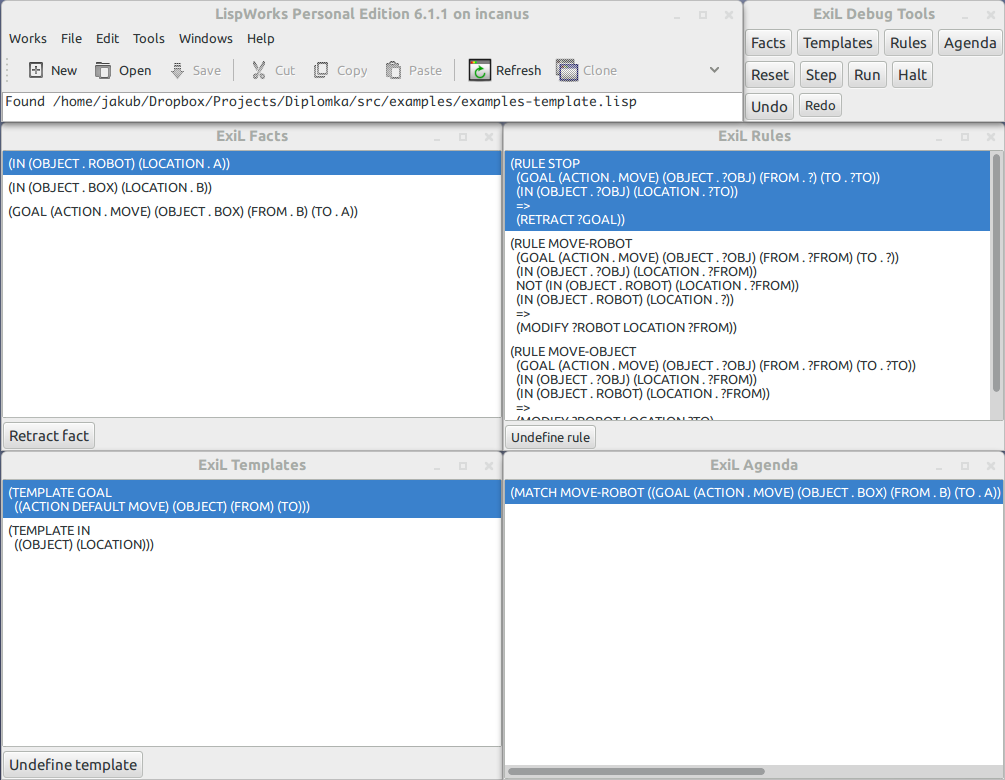
\includegraphics[width=\textwidth]{exil-gui.png}
\caption{Grafické uživatelské rozhraní}
\label{gui}
\end{figure}

Rozhraní lze zobrazit voláním \verb|(exil-gui:show-gui)|. Každé prostředí má
vlastní rozhraní. Volání \verb|show-gui| bez parametru zobrazí rozhraní k
aktuálnímu prostředí. Jako volitelný parametr můžeme funkci předat název
prostředí, jehož rozhraní chceme zobrazit. Máme-li tedy definováno více
prostředí, můžeme si ke každému z nich zobrazit uživatelské rozhraní.

